% CREATED BY DAVID FRISK, 2016
\chapter{Results}

\epigraph{ \textit{If you can not measure something, you can not improve it.}}{--- \textup{William Thomson Kelvin}}

\section{Evaluation metrics}
Generally speaking in Computer Science, every domain and application could have different evaluation metrics, for example the energy efficient of a CPU is a heavy metrics in embedded systems while in a high performant CPU latency and throughput are dominant metrics. As said that, evaluation metrics strongly depend on the end-users, therefore the designers have to make assumption on the end-user intentions and applications.\\
In this work the assumptions are that the accelerator will be deployed into an embedded system and at the same time it should give to the user a certain degree of flexibility for running Neural Network models. Thus, as it is suggested \cite{paper:1} the following metrics are used:
\begin{itemize}
\item Accuracy, quality of the final result of inference process.
\item Throughput, for measuring real time performance. It depends on the number of internal computation cores.
\item Latency, for interactive applications.
\item Energy and Power.
\item Hardware cost (Utilization Factor in case of an FPGA) of chip area and process technology.
\end{itemize}
\newpage
\section{Utilization Factor}
An important aspect of an embedded system is the on-die utilization area. Those kinds of system are usually deployed on tightly area constrained chips for hiding their presence to the user.
Therefore, it is important to measure and understand the behavior on the Utilization of the FPGA (used as area measurement in this case) of the design as the size of Matrix Multiplication Unit increases and in parallel the throughput.\\
The Utilization Factor, composed of Look-up-Table, Flip Flops and Digital Signal Processor usage, is expected to increase as the size of Multiplication Matrix increase and the bit width of Computation Unit.

In the following, utilization results are presented for each data type:
\begin{figure}[!htbp]
\centering
\captionsetup{justification=centering}
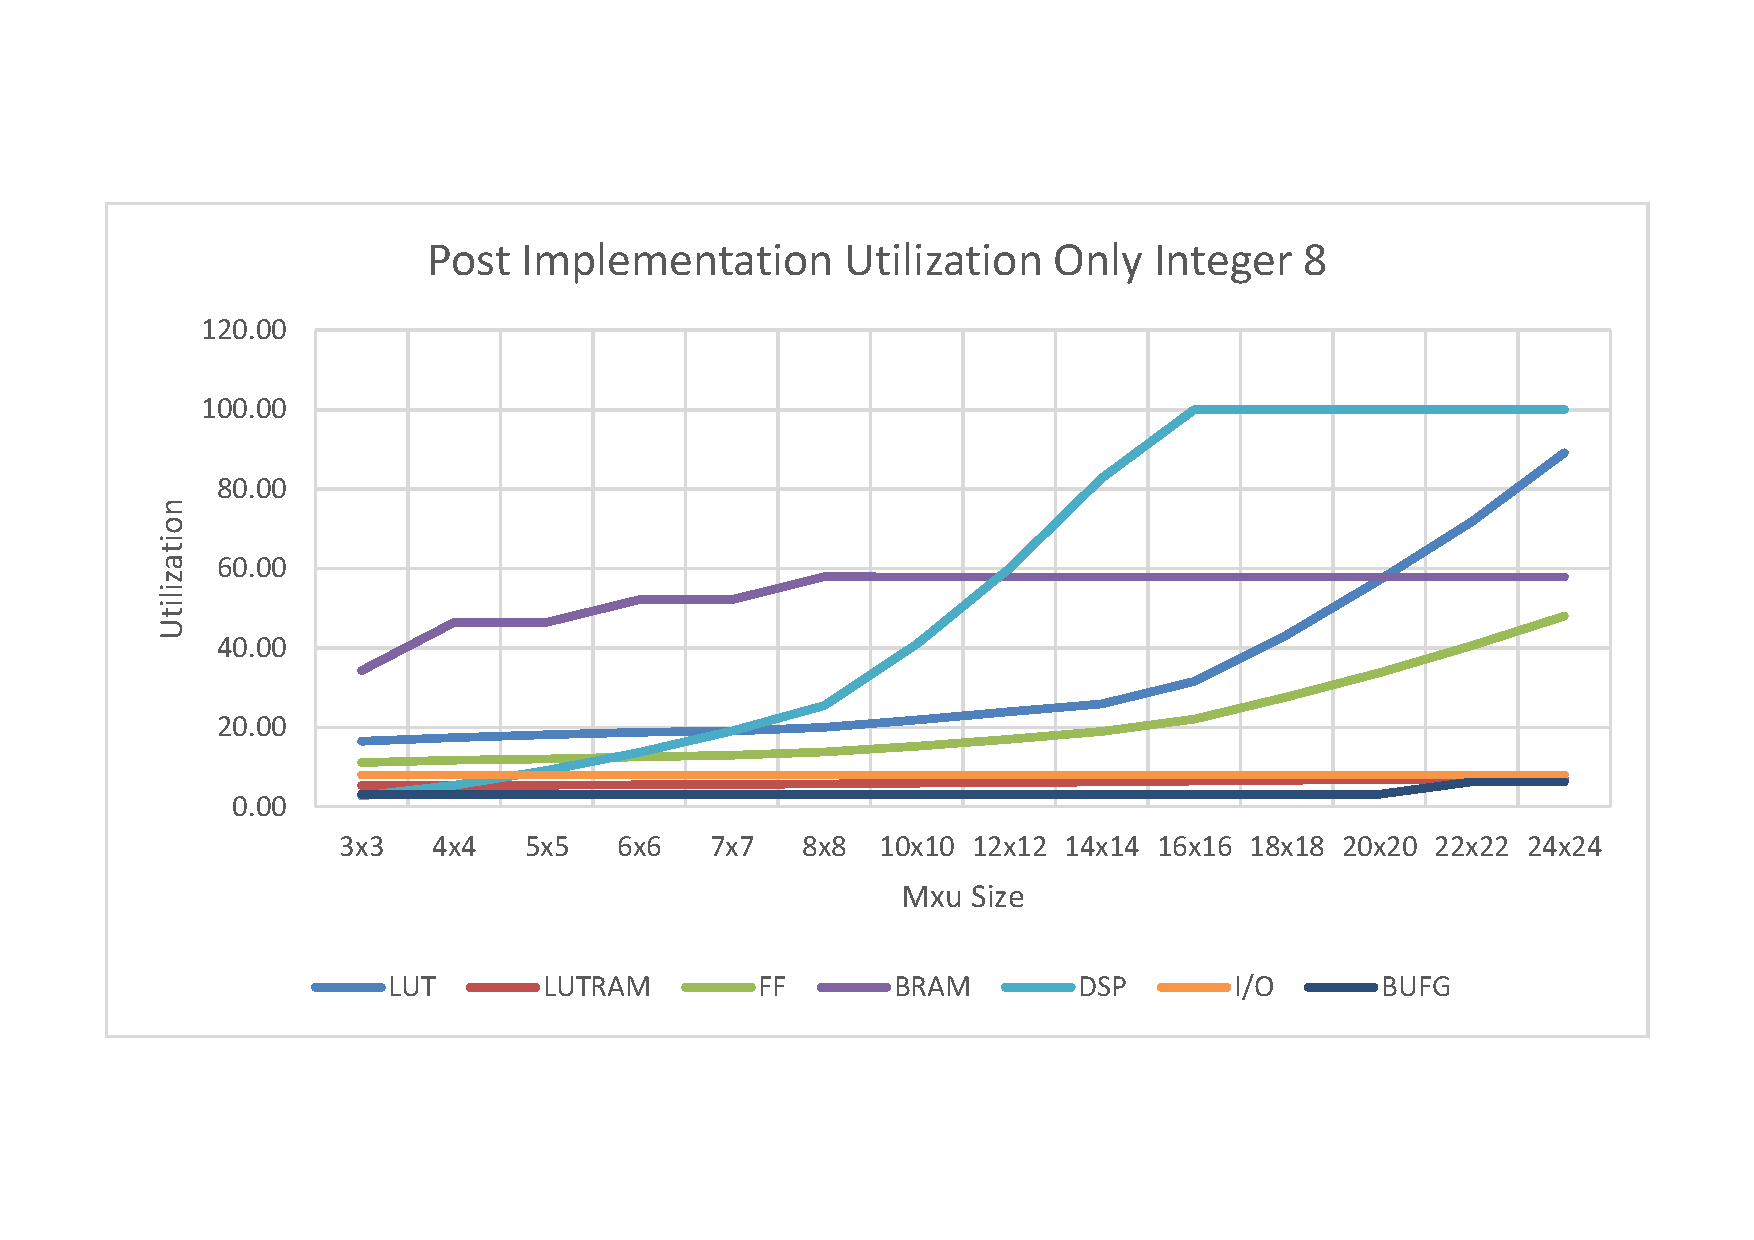
\includegraphics[scale=0.5,angle=0]{./figure/graphs/graph_utilization.pdf}
\label{fig:ut8bit}
\end{figure}

\newpage
\section{Energy and Power Consumption}
Energy and Power consumption are important factor, for a mobile device in which there is a limited battery capacity meanwhile for data centers stringent power ceilings due to cooling costs.

In the following, estimation of power consumption from Vivado are presented for each data type:

\begin{figure}[!htbp]
\centering
\captionsetup{justification=centering}
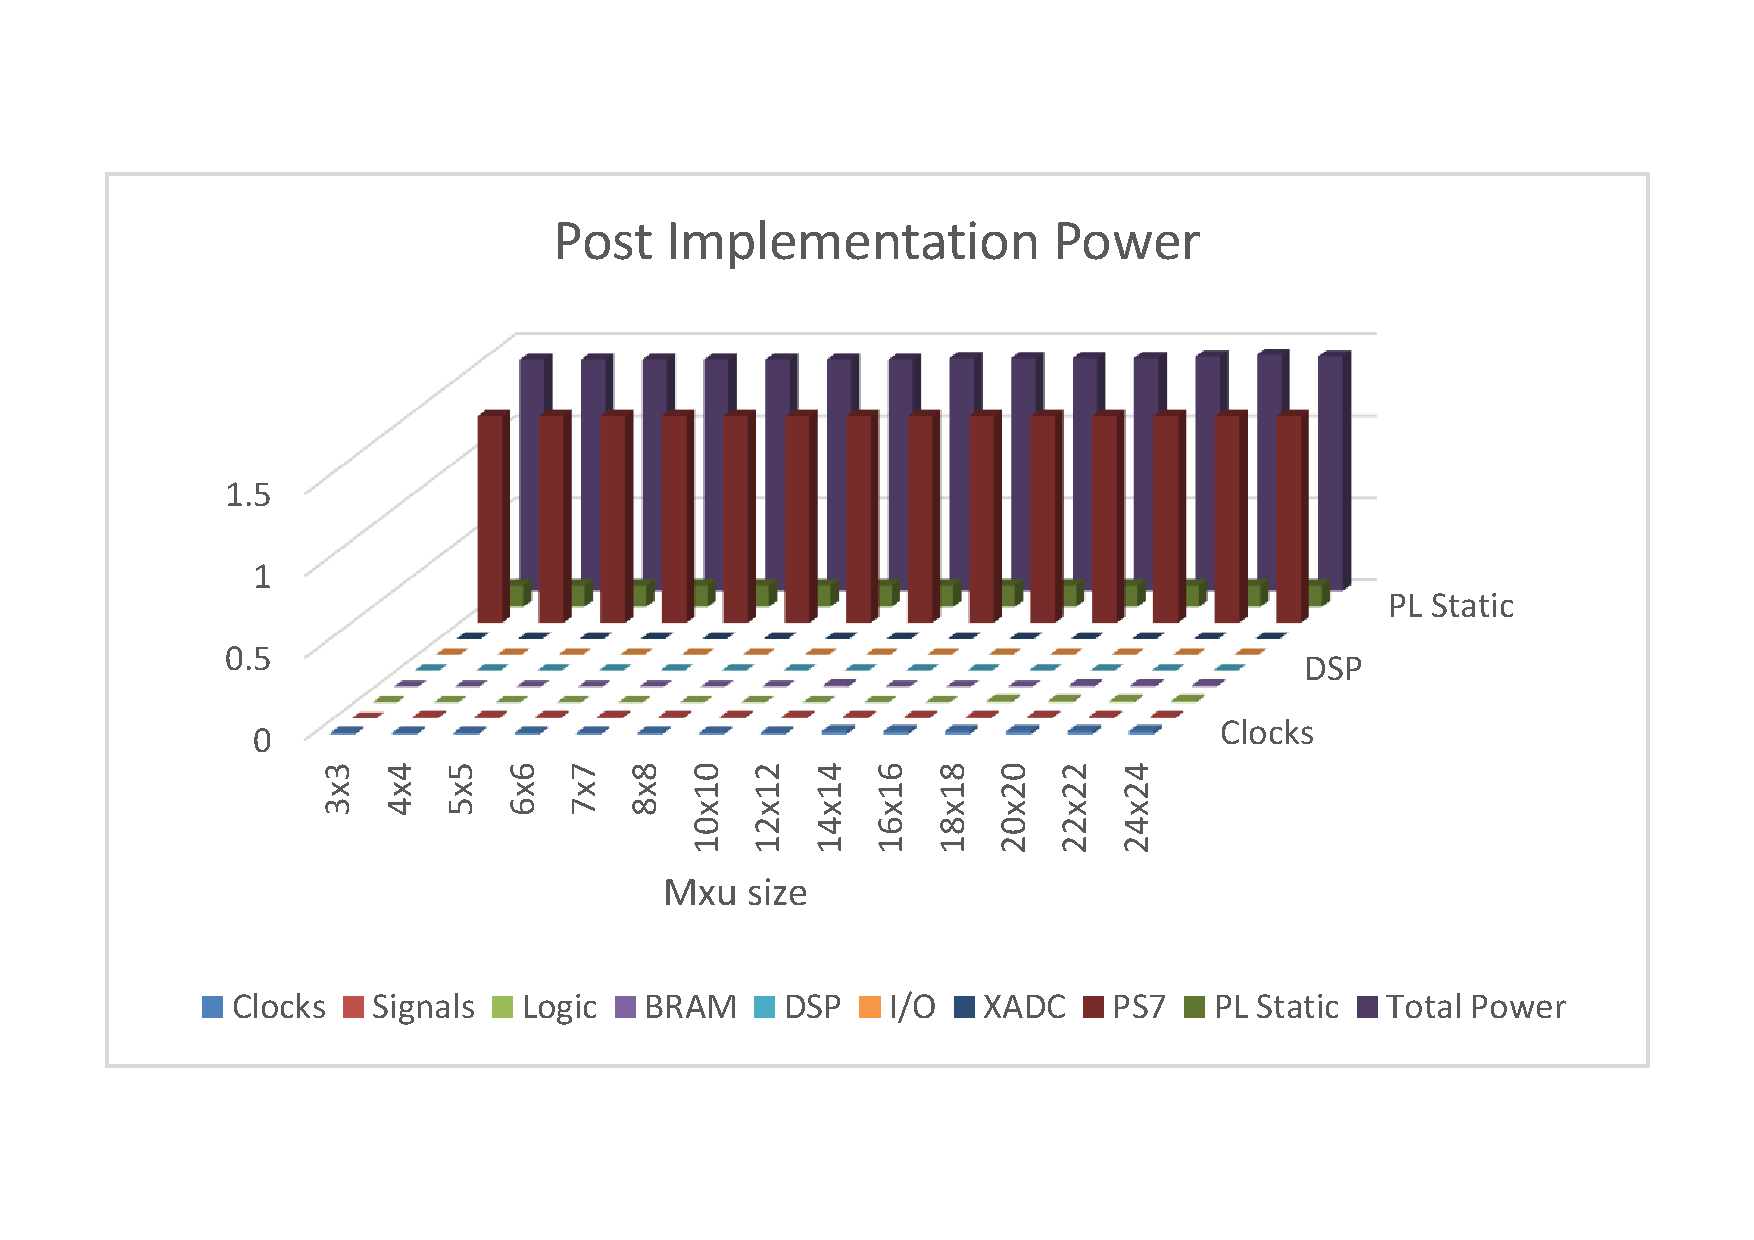
\includegraphics[scale=0.5,angle=0]{./figure/graphs/graph_power.pdf}
\label{fig:pow8bit}
\end{figure}

\newpage
\section{Throughput}
According to the definition, Throughput is the amount of units of information a system can process in a given time. As said that, for the designed accelerator it results to be equal to the number of rows into the Matrix Multiplication Unit. Normalizing this value with the clock frequency, it results to be constant for all the data type and frequencies:
\begin{figure}[!htbp]
\centering
\captionsetup{justification=centering}
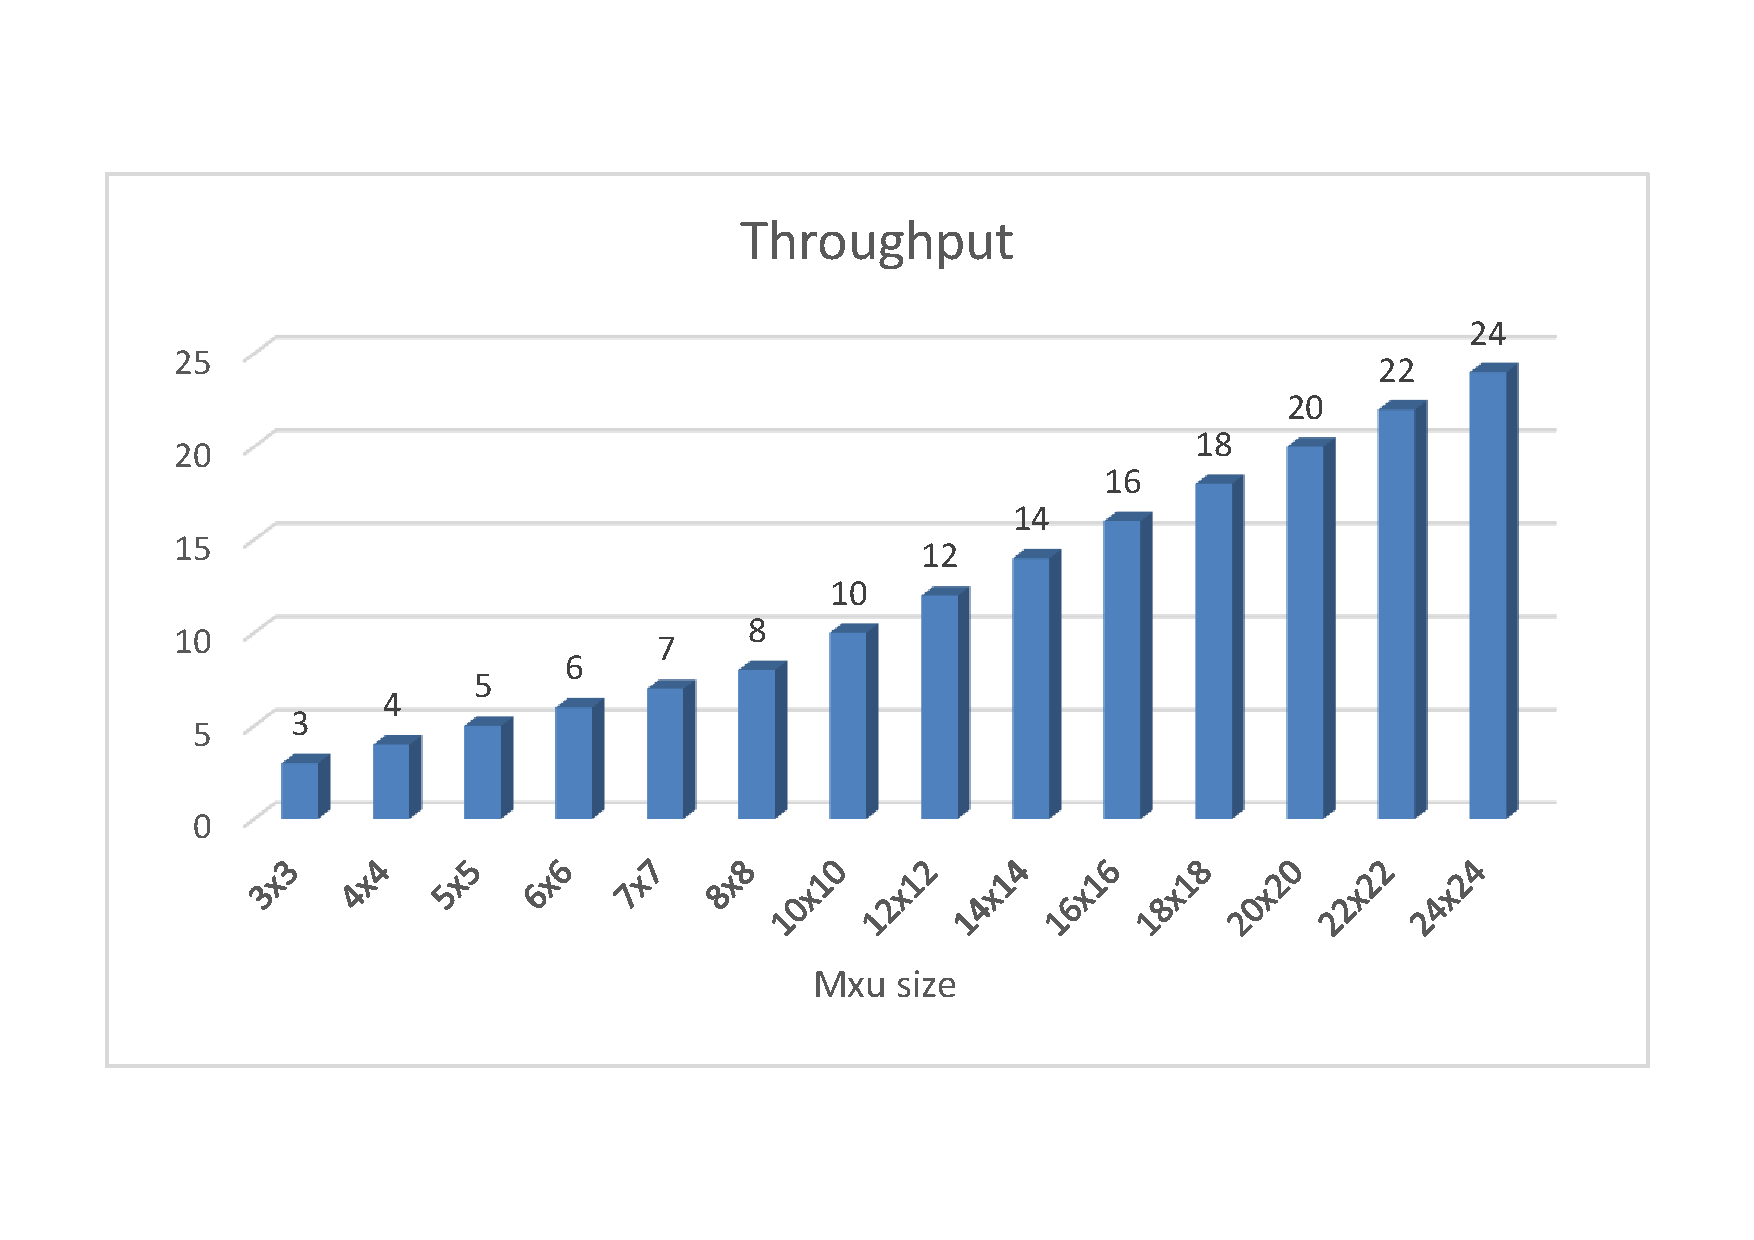
\includegraphics[scale=0.5,angle=0]{./figure/graphs/throughput.pdf}
\label{fig:tp8bit}
\end{figure}

\section{Latency}
In a real time application, the most important factor is the latency, the execution time of a task.
In this case the latency is measured as average of the execution time of a Neural Network model for different platforms. In addition, the execution of the models, on the target, in the configuration \textit{CPU+accelerator} is done with different clock frequencies and data type in the Programmable Logic, and as consequence a different overall latency (and power consumption).\\
In the following tables, the execution type for different data type and model is presented (with a fixed clock frequency of the accelerator at 80 MHz).
\begin{center}
\begin{table}[!htbp]
\centering
\captionsetup{justification=centering}
\begin{tabular}{ |p{2.5cm}||p{2.5cm}|p{2.5cm}|p{2.5cm}|p{2.5cm}| }
\hline
Model & CPU (host)\protect\footnotemark[1] & GPU(host)\protect\footnotemark[1] & CPU(Pynq Z2 board)\protect\footnotemark[3] & CPU(Pynq Z2 board) + accelerator \\
\hline
MNIST & 0.3 ms & 5.7 ms & 3.8 ms  & \\
\hline
Mobile Net V2& & 62 ms & &\\
\hline
Cifar 10& 20 ms & 22 ms& 343 ms &\\
\hline
\end{tabular}
\caption{Execution Time for different platform and model, integer 8}
\label{table:moplatint8}
\end{table}
\end{center}

\begin{comment}
\begin{center}
\begin{table}[!htbp]
\centering
\captionsetup{justification=centering}
\begin{tabular}{ |p{2.5cm}||p{2.5cm}|p{2.5cm}|p{2.5cm}|}
\hline
Model & CPU(Pynq Z2 board)\protect\footnotemark[3] & CPU(Pynq Z2 board) + accelerator & Speed-up \\
\hline
MNIST & 3.8 ms & ms &     \\
\hline
Mobile Net V2& & &\\
\hline
Cifar 10&  343 ms & ms &\\
\hline
\end{tabular}
\caption{Speed-up on target with accelerator for different models, integer 8}
\label{table:moplatint8}
\end{table}
\end{center}
\end{comment}




\todo{graph of how the execution time on the target changes with the frequency for every model}
\footnotetext[1]{Intel i7-6700HQ, 2.60 Ghz}
\footnotetext[2]{NVIDIA, GeForce GTX960M, 1.176 Ghz }
\footnotetext[3]{Arm dual-core Cortex-A9, 650 MHz }

On the other hand, the clock frequency of the accelerator can be tuned. Therefore, in the following, the behavior of the latency for every model with changing in the clock frequency is presented.

\newpage
\section{Accuracy}

\todo[inline]{list of NNs with the accuracy of the reference model(the one running on the board's cpu) with the cpu+accelerator run }

\begin{center}
\begin{table}[!htbp]
\centering
\captionsetup{justification=centering}
\begin{tabular}{ |p{3cm}||p{3cm}|p{3cm}|p{3cm}| }
\hline
Model & Reference Output \protect\footnotemark[1]& Actual Output\protect\footnotemark[2] & Relative Error\protect\footnotemark[3] \\
\hline
MNIST & & &\\
\hline
Mobile Net V1 integer8& & &\\
\hline
Mobile Net V1 fp32& & &\\
\hline
Cifar 10& & &\\
\hline
\end{tabular}
\caption{Accuracy Output of the and its relative error}
\label{table:accuracy}
\end{table}
\end{center}

\footnotetext[1]{Inference output of the model on the target, CPU only}
\footnotetext[2]{Target CPU + accelerator with MXU size of 8x8 and clock frequency at 80Mhz}

\footnotetext[3]{
$\epsilon _r=\Big|{\frac{OuputReference-ActualOutput}{OutputReference} }\Big|* 100 \% $
}

\section{Memory footprint}
\todo[inline]{ So having a chart or table with weight sizes (assuming this sis what is interesting to you since is what determines the local store of the FPGA engine) is enough. You should present the values for different bit length but no more.
As for the latency with frequency… it is always interesting to see if the applications is compute or memory bound (frequency changes the execution time r not?). So I would say include some results and also follow those for the energy evaluation (or efficiency).}